\section{Non-Functional Testing}

Non-functional testing is as important as functional testing since it is the basis for the quality of the product. It is important to ensure that the product is stable and reliable.

\subsection{Performance Testing} \label{sec:performance-testing}

One of the critical design goals of the system is to be able to use as few resources as possible while achieving all the functional requirements. To achieve this, the author used various techniques such as using system-level languages to write the core features and using modern coding practises such as coroutines to reduce resource waste.\\

\noindent The following diagram shows the relationship between the number of services that are being tracked versus the use of the system resource.

\begin{figure}[H]
    \centering
    \begin{subfigure}[b]{0.49\textwidth}
        \centering
        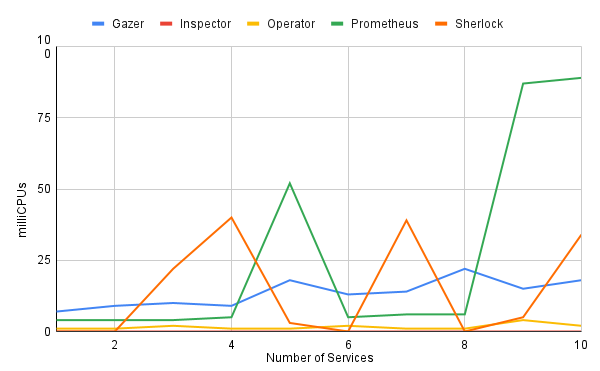
\includegraphics[width=8cm]{assets/testing/cpu-usage.png}
        \caption{CPU usage}
    \end{subfigure}
    \hfill
    \begin{subfigure}[b]{0.49\textwidth}
        \centering
        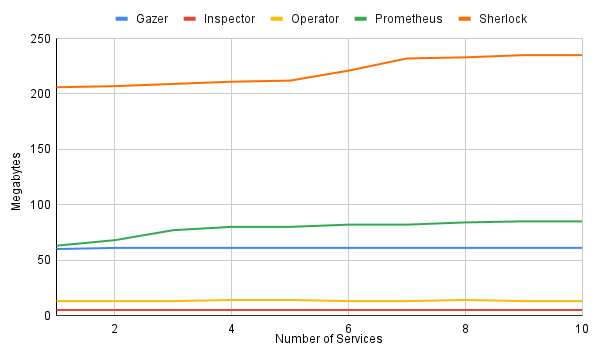
\includegraphics[width=8cm]{assets/testing/memory-usage.png}
        \caption{Memory usage}
    \end{subfigure}
    \hfill
    \caption{Resource Usage vs Number of Services (self-composed)}
\end{figure}


\subsection{Usability Testing}

To increase the adaptability and usability of the system the author undertook a number of steps

\begin{itemize}
    \item As shown in Section \ref{sec:module-integration-testing}, all the components of the system are designed in a way that allows users to install individual components and still make use of them effectibly.
    \item Even though most of Kubernetes tooling revolved around terminals, for this system the author has created an intuitive UI so that users can interact without having to go though long documentations.
    \item The service graph is designed to be easily navigable and to allow users to easily find the relevant services.
    \item The entire application was packaged as a helm chart so the end-users can deploy or removed it to their cluster using a single command.

\end{itemize}

\noindent During the evaluation phase, the author demonstrated the end-to-end behaviour of the system and asked the evaluators to rate the usability of the system. The results of that are shown below.


\begin{figure}[H]
    \centering
    \begin{subfigure}[bH]{0.49\textwidth}
        \centering
        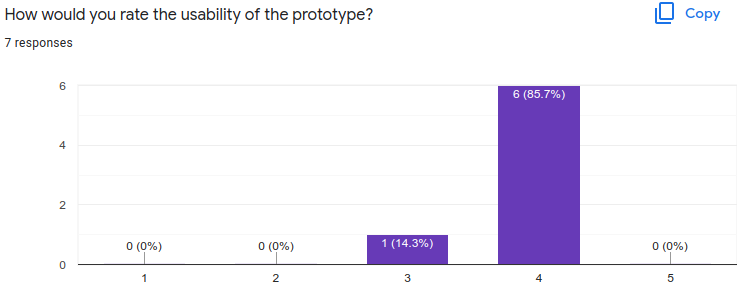
\includegraphics[width=8cm]{assets/testing/usability.png}
    \end{subfigure}
    \hfill
    \begin{subfigure}[bH]{0.49\textwidth}
        \centering
        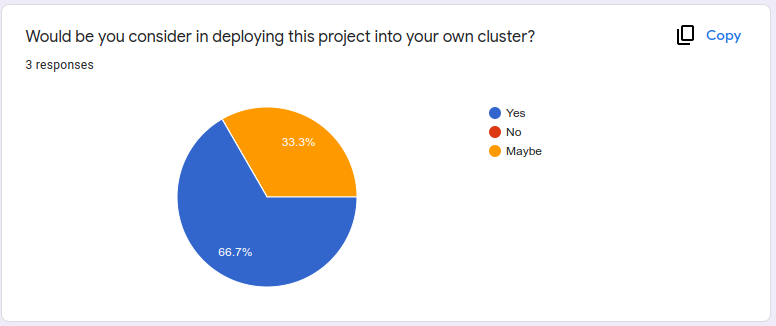
\includegraphics[width=8cm]{assets/testing/use-or-not.png}
    \end{subfigure}
    \hfill
    \caption{Usability of the system as rated by evaluator (self-composed)}
\end{figure}




\subsection{Maintainability and Adaptability Testing}

The main proposal of this project is to provide a framework for the research community to develop to push the limits of \ac{aiops}. So, from the very beginning, the system was consciously designed in a way that is easy to maintain and can be easily extended. Since quantifying the results of these effort is difficult, the author asked the evaluators number of questions to gauge the maintainability and adaptability of the system. The results of that are shown below.

\begin{figure}[H]
    \centering
    \begin{subfigure}[bH]{0.49\textwidth}
        \centering
        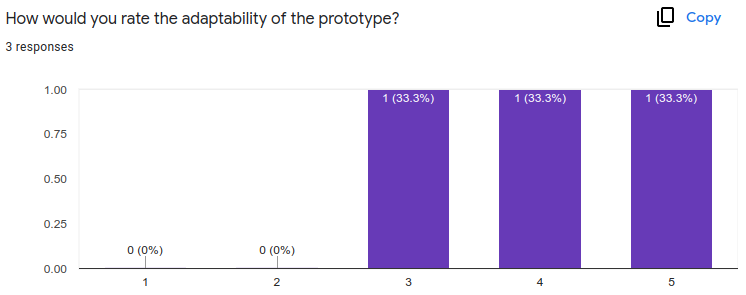
\includegraphics[width=8cm]{assets/testing/adaptability.png}
    \end{subfigure}
    \hfill
    \begin{subfigure}[bH]{0.49\textwidth}
        \centering
        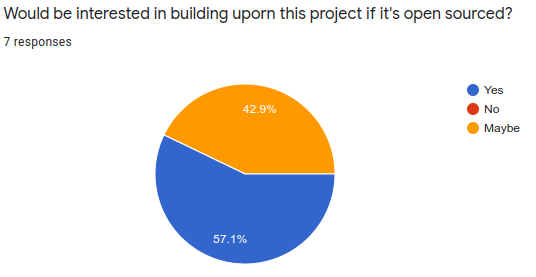
\includegraphics[width=8cm]{assets/testing/build-uporn.png}
    \end{subfigure}
    \hfill
    \caption{Maintainability and adaptability of the system as rated by evaluator (self-composed)}
\end{figure}


\subsection{Generalisation Testing}

Deep learning component of this system is based on the idea that at a fundamental level, all service acts the same. So, the author collected telemetry data from all services and trained a single model to understand the behaviour of the system. Once that based model is trained, it was fine tuned on the data collected from each service so the model get specialized to that particular service.

\begin{figure}[H]
    \centering
    \begin{subfigure}[bH]{0.49\textwidth}
        \centering
        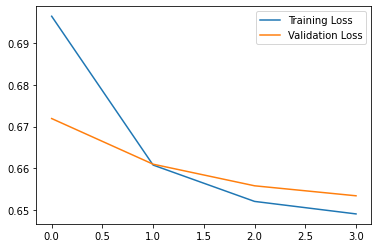
\includegraphics[width=8cm]{assets/testing/loss-base-model.png}
        \caption{Training loss of the base model}
    \end{subfigure}
    \hfill
    \begin{subfigure}[bH]{0.49\textwidth}
        \centering
        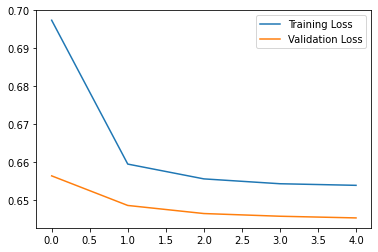
\includegraphics[width=8cm]{assets/testing/loss-service-2.png}
        \caption{Training loss of a specialized model}
    \end{subfigure}
    \hfill
    \caption{Generalizability of the Autoencoder (self-composed)}
\end{figure}